\documentclass[../master.tex]{subfile}
\begin{document}

\section{Analysis}
Our goals for this final deliverable is stated down below. This section will explain these goals, the relevance of them and what specifications that are required in this project.
\label{sec:Goals}

\subsection*{Goal 1: Meeting the requirements}
\label{sec:Goal1}
This goal is one of the most important goals we have. It concerns about the functionality and requirements of our game. It helps us making sure that our game moving towards a playable game. We need to meet the \hyperref[sec:Requirements]{requirements} of the \textit{deliverables} 7-10, which all sum up to be the finished game.

\subsection*{Goal 2: Design patterns}
This goal concerns utilizing sensible design patterns, where they are relevant. In software development, a design pattern is a general, and reusable solution to a commonly occurring problem within a given context in software design. There exists many different design patterns and each of them are used for different things, while some also recalls other patterns. The approach of using a design pattern can be rewarding for the code quality and can help solve a given problem. The approach can be recognized by many other developers who have to read, understand and edit the code, which also helps supporting \hyperref[sec:Goal3]{goal 3} and \hyperref[sec:Goal6]{goal 6}, as it standardizes the code. This is one of our goals, since we have to research different design patterns and get to learn using them in some different occasions.

\subsection*{Goal 3: Maintainability}
\label{sec:Goal3}
This goal concerns making the code maintainable, understandable and accessible to other developers who may want to change it. This can be achieved by using names that is appropriate to what each method, class or variable is meant to do. By writing a good documentation will also allow readers to form better mental overview over any solution, and will together with explicit names create a code, that is much more readable. Then updating the code it may also fix flaws thay may be hiding in the program. By keeping the SOLID principles in mind, when designing it will also do much for the maintainability of the code.\\

The maintainability of this project is a very important part of the development for us, as we are developing the project in a group. We have been sitting together during the designing of the code, and communicated about the design and the quality, ensuring that the code would be readable by everyone in the group. This was important since we were working on differnt parts of the code at the same time. In this deliverable we will return to old pieces of code, which we have to refresh our minds with and do some refactoring, that will make it easier for other people to read.

\subsection*{Goal 4: Tests}
\label{sec:Goal4}
This goal concerns tests. Tests can be coded to ensure that methods and classes actually do what they are supposed to do. Tests are also able to help exposing if there are any bugs located in the code. By having tests which checks troughout the program, that the units of the code functions as intended will improve maintainability, and it supports \hyperref[sec:Goal3]{goal 3}. If new changes are made, any unintended effects should be caught by the test. That means all classes that we have written requires testing, except the game class, as this heavily relies on the GaneEventBus (has already been tested). The code should also be designed, so methods and classes are suitable for unit-testing.

\subsection*{Goal 5: Design for extensibility}
This goal concerns designing the project for further extensibility. Extensibility is a software development and systems design principle where the implementation takes future growth into consideration. The goal here is to accomodate for expected future additions to avoid the need for some major refactoring in order to include additions to the program, while also maintaining a reasonable structure.

\subsection*{Goal 6: Coding style}
\label{sec:Goal6}
In this project we should stick to a specific guideline for coding style and naming. This will in many cases, help readers to get an better overview of a code. By using one guideline it also helps ourselves as it will keep away unnecessary confusion which may or may not lead to errors. In our group we have done our best to follow the guideline provided to us, as well as to follow the naming guidelines which are stated by the .NET Framework Naming Guidelines. This goal impacts on readability, which also supports \hyperref[sec:Goal3]{goal 3}.

\subsection{Requirements for Space Taxi}
\label{sec:Requirements}
For the game including this project, it is needed to have a player-taxi that can be controlled by the player. The ship should be affected by the laws of physics, which consists of: When accelerating upwards and sideways it should be accelerating gradually, which means as it is in space it should go faster and faster the longer the player holds down the keys to the left, right or up, also while its being affected by gravity. When the player stops pressing the up-key, which is accelerating the player-ship upwards, the ship should gradually start to fall. The fall should have the same accelerating features as when pressing the left, right or up key, but as it is falling due to gravity, this will go faster than the acceleration from the thrusters. To de-accelerate from the fall when pressing the up-key it should as well de-accelerate gradually. This will overall simulate the laws of physics and gravity. The player should as well be able to pick up customers by landing on platforms and then fly them to their desired next platform, where they will be dropped off and disappear. By ``delivering`` customers it should give the player money (points basically). It is also needed to have a timer showing frames and updates pr. second, as well as an event handler, and a state machine which will handle different states in the game, as then the player are put into the main menu or teleporting to another level. Or other examples as: when the game is running, pausing the game and quitting the game.\\

This is some of the things, that is needed to make Space Taxi. The frame of the game can contain:
\begin{enumerate}
	\item Start the game.
	\item Starts in the main menu, where user inputs can be accepted as ("Key up", "key down" and "key Enter"), to start a new game or quit the game.
	\item When starting the game, draw and render game elements (background, objects, obstacles, platforms teleportation device in the top middle screen to change level and player-taxi.
	\item Position the player ship up in the right corner, beside the sugar cane on the left side. Accept user inputs (key-left, key-right and key-up).
    \item Position customer, which can be picked up at a platform and dropped off on a next one.
	\item Depending on the user input, handle the event, change the game state, draw the next frame.
\end{enumerate}

The game should be a single-player game, where the player will be introduced with a main-menu screen. Here the player should be able to select between starting a ``New Game`` and a ``Quit`` game button, as you then will have what is needed for a functional working game. The game should be able to quit the game as you hit the quit button, as well start a new game, then hitting the ``New Game`` button. Then pressing the ``New Game`` button, the game should start and the player will be put into the game. Here should the player start in the first environment ``Short-n-Sweet``, which technically should work as the first level. Here the player should see the player-ship (the space taxi), that can be moved left, right and upwards by using the keys for left, right and up. The player will also be able to pick up customers at platforms and deliver them to their desired next platform, and by that earn money. The game should run with 60 frames pr. second and have 60 Updates pr. second, as well as be fast and responsive then hitting the buttons. If not, it will be annoying for the player if the buttons does not response immediately, as it will make the game frustrating when you want to de-accelerate at the right moment to avoid hitting obstacles, which will cause the ship to explode. To go to the next level, the player should be able to ``collide`` with the portal in the top middle of the screen and then get teleported to the next level ``The Beach``.\\

To interact with the main-menu and the game, the game needs the implementations:\\
For instance, to interact with the menu:\\
\begin{wrapfigure}{l}{0.03\textwidth}
	\vspace{-1.8mm}
	\begin{centering}
		
\includegraphics[width=0.04\textwidth]{./Pictures/Pil_op.png}
	\end{centering}
	\vspace{-6mm}
\end{wrapfigure}
Go one choice up, if possible.\\

\begin{wrapfigure}{l}{0.03\textwidth}
	\vspace{-5.8mm}
	\begin{centering}
		
\includegraphics[width=0.04\textwidth]{./Pictures/Pil_ned.png}
	\end{centering}
	\vspace{-6mm}
\end{wrapfigure}
Go one choice down, if possible.\\

\begin{wrapfigure}{l}{0.03\textwidth}
	\vspace{-5.8mm}
	\begin{centering}
		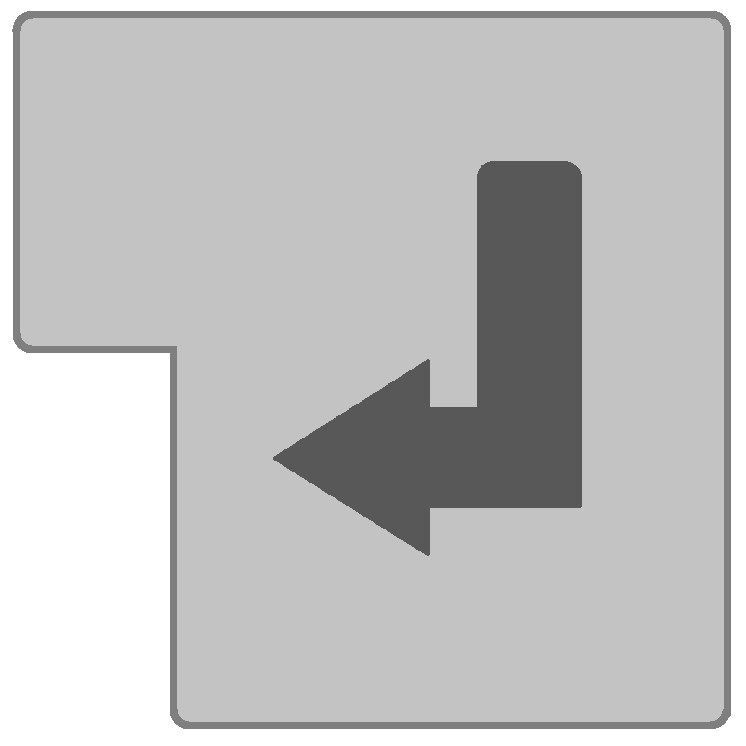
\includegraphics[width=0.04\textwidth]{./Pictures/Enter.png}
	\end{centering}
	\vspace{-6mm}
\end{wrapfigure}
To select your chosen menu button press enter, if possible.\\

When the player chooses ``New Game``, the game should start, while if the player chooses ``Quit``, it will Quit the game. When the game starts, the player should see the ship placed in the top right corner of the screen on the left side of the sugar cane. The player will also be seeing the level itself, containing a background, walls, obstacles, the portal and the platforms that can be used to land on and pick up costumers as well as deliver customers at. The player should be able to move the ship to left, right and upwards, while also noticing that the ship is being affected by physics. Furthermore, the player should be able to go to the next level by using the teleporter in the top middle of the screen. To make this happen, if possible it is needed to implement, the following keys:\\
\begin{wrapfigure}{l}{0.03\textwidth}
	\vspace{-6mm}
	\begin{centering}
		
\includegraphics[width=0.04\textwidth]{./Pictures/Pil_op.png}
	\end{centering}
	\vspace{-6mm}
\end{wrapfigure}
Will accelerate the ship upwards, if possible.\\

\begin{wrapfigure}{l}{0.03\textwidth}
	\vspace{-6mm}
	\begin{centering}
		
\includegraphics[width=0.04\textwidth]{./Pictures/Pil_venstre.png}
	\end{centering}
	\vspace{-6mm}
\end{wrapfigure}
Will accelerate the ship to the left, if possible.\\

\begin{wrapfigure}{l}{0.03\textwidth}
	\vspace{-6mm}
	\begin{centering}
		
\includegraphics[width=0.04\textwidth]{./Pictures/Pil_right.png}
	\end{centering}
	\vspace{-6mm}
\end{wrapfigure}
Will accelerate the ship to the right, if possible.\\

If possible the player should also be able to pause the game using the ``P`` key on the keyboard, where the player should be able to quit the game by pressing the Q-key and start a new game by pressing the N-key. To make this possible it is needed to implement the following things:\\
\begin{wrapfigure}{l}{0.03\textwidth}
	\vspace{-5.9mm}
	\begin{centering}
		
\includegraphics[width=0.04\textwidth]{./Pictures/Pause.png}
	\end{centering}
	\vspace{-6mm}
\end{wrapfigure}
Hit the P-key to pause the game, if possible.\\

\begin{wrapfigure}{l}{0.03\textwidth}
	\vspace{-5.9mm}
	\begin{centering}
		
\includegraphics[width=0.04\textwidth]{./Pictures/Quit.png}
	\end{centering}
	\vspace{-6mm}
\end{wrapfigure}
After hitting P-key, press Q to quit the game, if possible.\\

\begin{wrapfigure}{l}{0.03\textwidth}
	\vspace{-6mm}
	\begin{centering}
		
\includegraphics[width=0.04\textwidth]{./Pictures/New_Game.png}
	\end{centering}
	\vspace{-6mm}
\end{wrapfigure}
After hitting P-key, press N to start a new game, if possible.\\

Design goals relating to technology stack choices:
\begin{enumerate}
	\item The game should be written in C\#, as a JetBrain Rider project, version controlled with Git - the technology stack of our course.
	\item The game should run across the different operating systems. 
\end{enumerate}

Design goals relating to coding style:
\begin{enumerate}
	\item The game needs to be made using the game-engine DIKUArcade.
	\item The game should be able to handle the player being affected by physics, when the player-ship collides with an obstacle, when it should land on a platform, and when going to the next level. It should draw and render the game and its elements according to the different game states. 
	\item The game should be designed such that the GameEventBus can be accessed through a GetBus method, so we can access the same GameEventBus from anywhere in our program, and not only in the Game class. Which means that the game should be designed, so we can handle events anywhere in our program.
	\item The program should be designed such as, instead of having all of the methods which relates to the player class inside the Game class, it should be in a class of its own named "Player".
	\item The game should be designed so it has a state machine, that will handle the different states, such as when game is in the main menu, when the game is running, when the game is paused and quit game. As well when the ship collides with obstacles, it should explode, when it comes near a platform, it should land and when it collides with the teleporter, it should change the level. Furthermore, be able to transition between the different states, changing which state is active.
\end{enumerate}

\end{document}